% !TeX root = ../summary-syssec.tex
\section{Stack Attacks}
\subsection{Stack Frame}
\begin{center}
  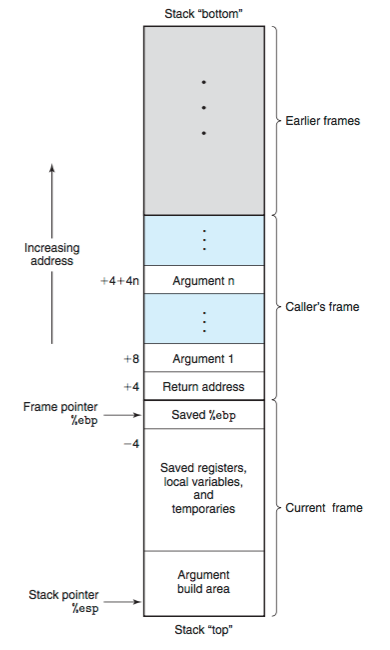
\includegraphics[width = 0.5\columnwidth]{stack-frame-structure.png}
\end{center}

\subsubsection{Construction}
The steps needed to call a function and construct a new stack frame are
\begin{enumerate}
  \item Push the last argument to the top of the stack;
  \item Push the first argument onto the stack;
  \item Push the return address onto the stack;
  \item Jumping to the called function;
  \item Saving the caller's base pointer on the stack;
  \item Move the base pointer to the top of the stack
  \item Allocating local memory for the callee.
\end{enumerate}

\subsubsection{Destruction}
The steps needed to seamlessly return and resume the execution of the parent
(caller) function are:
\begin{enumerate}
  \item Moving the stack pointer to the bottom of the callee's frame (value of
    \texttt{ebp})
  \item Restoring the caller's base pointer by popping it
  \item Taking the return address off the stack and jumping to it
  \item Freeing space allocated for the callee arguments
\end{enumerate}

\subsection{Protection}
\begin{description}
  \item[Canaries:] A known value that should never change is saved on the
    stack. If the value is checked and is not the value it should be, the
    system can conclude that there was a buffer overflow.
  \item [Address space layout randomization (ASLR):] The addresses of
    stack, heap and libraries are moved around. Because of this, the
    addresses of specific calls are different on every call, and
    attacker can't find the correct address by trial and error.
\end{description}

\subsection{Format String attacks}
A program such as
\begin{lstlisting}
int main (int argc, char** argv) {
   char *name = argv[1];
   printf(name);
}
\end{lstlisting}
is vulnerable to format string attacks. Interesting inputs are:
\begin{description}
  \item[\texttt{printf(\%s)}:] This will lead the program to print out parts of
    the memory.
  \item[\texttt{printf(\%n, \&i)}:] Writes the number of characters printed so
    far to the address \texttt{\&i}.
\end{description}

